\chapter{自然语言处理}
\begin{introduction}
  \item Attention Mechanism
  \item Transformer
  \item BERT
  \item GPT
  \item Bi-Encoder
  \item Cross-Encoder
\end{introduction}

\section{注意力机制 (Attention Mechanism)}


\subsection{为什么要用多头注意力机制?}

通俗的解释是,多头注意力机制会学习不同的 Q、K、V 子空间,因而能够将这种不同维度的信息综合起来,使得模型有更好的表征能力。这里也可以参照cs224n中\href{https://web.stanford.edu/class/cs224n/assignments/a5.pdf}{ assignment5 }举的例子来解释:多头注意力机制对于K的长度变化更加不敏感,因而增强了模型的鲁棒性和泛化能力。

\section{Transformer}

\begin{figure}[htbp]
  \centering
  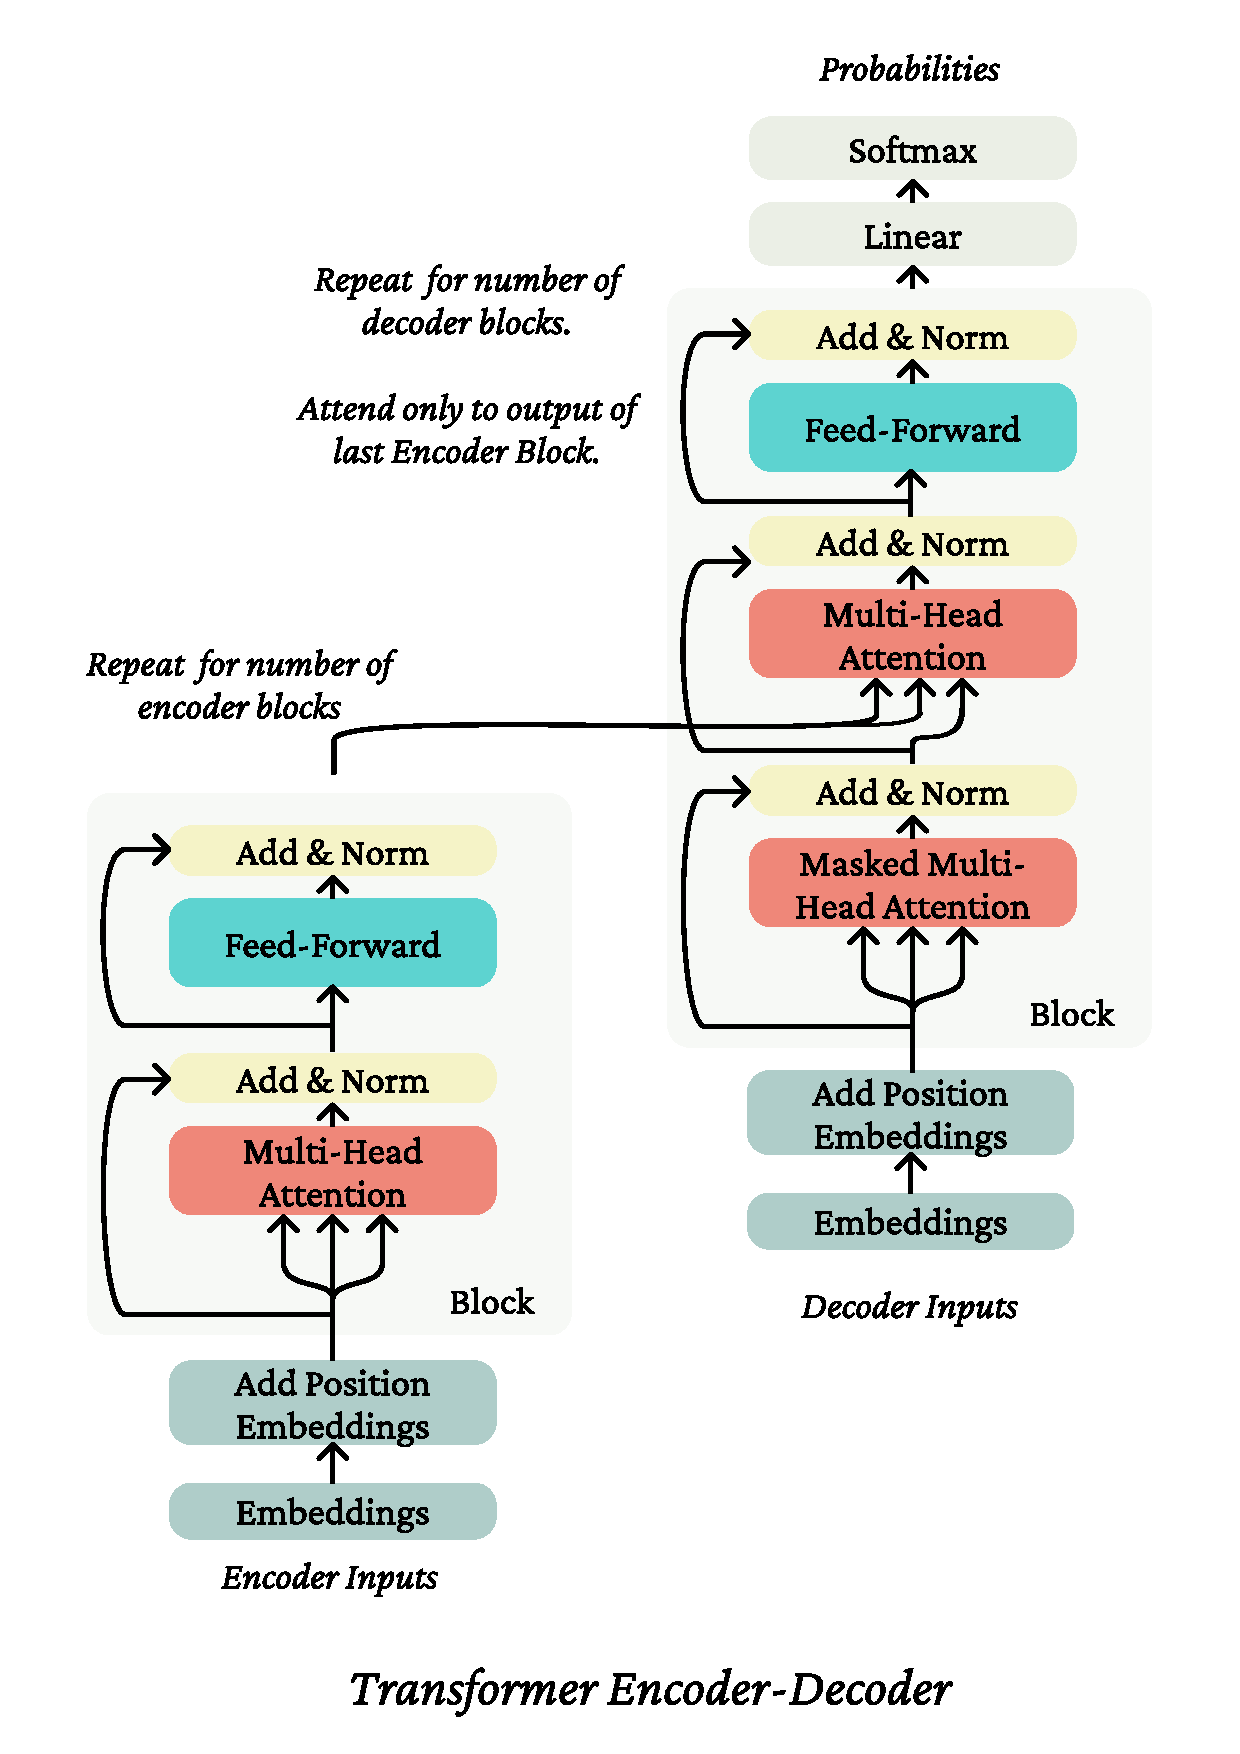
\includegraphics[width=0.6\textwidth]{transformer.pdf}
  \caption{Transformer架构 \label{fig:transformer}}
\end{figure}


\subsection{Batch Normalization 还是 Layer Normalization?}

\section{基于BERT的检索模型}

本章节将介绍两种业界常见的基于BERT的信息检索(Information Retrieval)模型:Bi-Encoder和Cross-Encoder。其中Bi-Encoder是双塔结构,主要用于信息的召回阶段;Cross-Encoder为单塔结构,主要用于召回后的精排或者粗排。

\subsection{Bi-Encoder}

双塔结构广泛应用于推荐和搜索场景,由于该模型结构能够解耦合查询的query和待查询的document pool或者用户与待推荐的商品集合。我们下面以搜索场景介绍:当模型训练完成后,我们对document pool中的所有document进行模型推理。得到embedding后构建近似搜索的索引。当新的query产生,双塔模型中的query tower将进行inference生成embedding。我们即可用此embedding在document embedding index中检索。搜索模型中双塔模型想要达到比较好的效果,在以下几个方面需要有所考量:

\subsubsection{负样本采样}

负样本采样的“招式”很多,既有in-batch negative sampling,又有offline hard negative mining。其中,in-batch 的负样本采样指的是对于某个正例样本组$(q,d_+)$,我们可以将在模型训练过程中同一个batch内的其它样本组的document取出作为负样本。可以取一部分,例如按照$q$与负样本的score来排序截取。也可以全部拿来作为负样本使用。

Offline hard negative mining 相对复杂一些:根据当前模型从document集合中召回样本,剔除其中包含的正例样本。这也是其中"negative"的由来,因为按照此法得到的document实为与$q$很相关但又没有被用户所点击。这里涉及到一个False Negative的问题,

\subsubsection{对比学习}






\subsection{Cross-Encoder}
